\section{Architecture and Pipeline Overview}\label{sec:overview}

Our model is an agentic system assembled in two stages: (i) from-scratch pre-training of a hybrid language backbone, and (ii) post-training of that backbone (instruction tuning and reinforcement learning to strengthen agentic capability).
% 中文：本模型是一个由两个阶段组装而成的智能体系统：(i) 从零预训练混合语言骨干；(ii) 对该骨干做后训练（指令微调与强化学习以增强智能体能力）。
At deployment, the model is a subagent in a star topology: a central orchestrator holds the user's intent and dispatches each subtask to the subagent of the relevant EDA tool, which translates the subtask into that tool's native script (PyAether, SKILL, Tcl) and operates the tool locally.
% 中文：部署时，本模型在星型拓扑中作为子智能体运行：中央 orchestrator 把握用户意图，把每个子任务分派给相关 EDA 工具的子智能体，由后者把子任务翻译成该工具的原生脚本（PyAether、SKILL、Tcl）并在本地操作工具。
This section fixes the shared scaffolding---the backbone, the overall pipeline, and the global training environment---before each stage is detailed in its own section.
% 中文：本节先固定各部分共享的脚手架——两个骨干网络、整体流水线与全局训练环境——随后各阶段再在各自章节中详述。

\subsection{Language Backbone}\label{sec:arch}
The language backbone is a sequential hybrid model~\cite{dao2024transformers,nvidia2025nemotronh}: 56 transformer layers interleave Mamba-2 state-space layers, four grouped-query-attention (GQA) layers, and MLP layers.
% 中文：语言骨干。语言骨干是一个顺序式混合模型 \cite{dao2024transformers,nvidia2025nemotronh}：56 个 transformer 层交替排列 Mamba-2 状态空间层、4 个分组查询注意力（GQA）层与 MLP 层。
The layer allocation follows the Nemotron-H sequential hybrid convention---four attention layers among the 56, the remainder Mamba-2 and MLP---as provided by Megatron-Core's Mamba-hybrid recipe, whose 56-layer pattern we reuse verbatim while halving only the hidden and FFN widths to reach the $\approx$2B scale.
% 中文：层的分配遵循 Nemotron-H 的顺序式混合约定——56 层中 4 层为注意力，其余为 Mamba-2 与 MLP——由 Megatron-Core 的 Mamba 混合配方给出；我们原样复用了其 56 层模式，仅将隐藏维度与 FFN 宽度减半以达到约 2B 规模。
Our model is not a Nemotron-H model: it is an order of magnitude smaller, contains no mixture-of-experts layers, and is pre-trained from scratch on an independent corpus under a fixed GPU-hour budget.
% 中文：本模型并非 Nemotron-H 模型：它小了一个数量级，不含专家混合（MoE）层，并在固定 GPU·h 预算下于独立语料上从零预训练。
Each Mamba-2 layer uses 8 state-space groups; the four attention layers use 16 query heads and 4 query groups (GQA) with untied word embeddings.
% 中文：每个 Mamba-2 层使用 8 个状态空间组；4 个注意力层使用 16 个查询头与 4 个查询组（GQA），且词嵌入不共享。
Crucially, only the four attention layers carry rotary position embeddings (RoPE); the 52 non-attention layers (24 Mamba-2 SSM and 28 MLP) are position-agnostic, so the backbone's long-context extrapolation quality depends on just $4/56{=}7.1\%$ of layers, an asymmetry exploited in Section~\ref{sec:longctx}.
% 中文：关键在于，只有 4 个注意力层携带旋转位置编码（RoPE）；其余 52 个非注意力层（24 个 Mamba-2 SSM 与 28 个 MLP）与位置无关，因此骨干的长上下文外推质量仅取决于 $4/56{=}7.1\%$ 的层——这一不对称性在第 \ref{sec:longctx} 节被加以利用。
The full configuration is listed in Table~\ref{tab:config}; the model totals $\approx$2.22B parameters.
% 中文：完整配置见表 \ref{tab:config}；模型参数量约 22.2 亿。
Figure~\ref{fig:backbone} illustrates the layer interleaving: the four attention layers (with RoPE) are the only layers whose memory grows with session length, while the 52 Mamba-2 SSM and MLP layers maintain a fixed-size recurrent state.
% 中文：图 \ref{fig:backbone} 展示了层的交错排列：4 个注意力层（带 RoPE）是唯一随会话长度增长内存的层，而 52 个 Mamba-2 SSM 与 MLP 层维持固定大小的递归状态。

\begin{figure}[t]
\centering
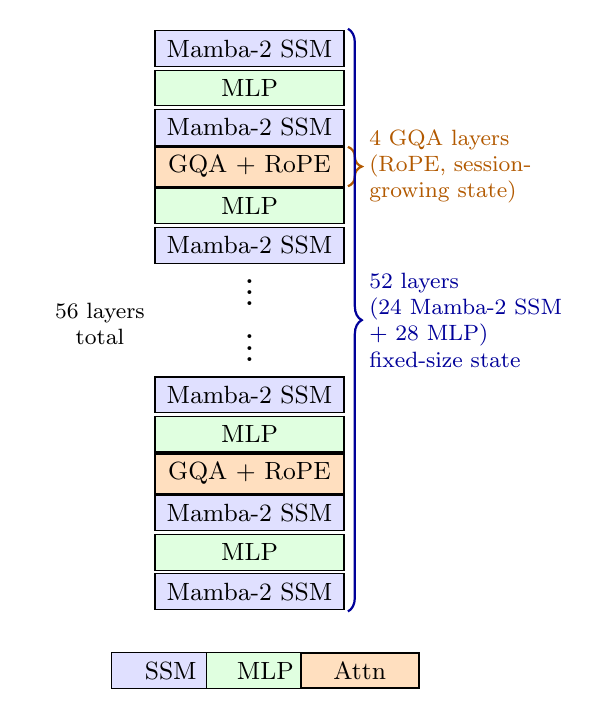
\begin{tikzpicture}[
  layer/.style={draw, minimum width=2.4cm, minimum height=0.42cm, font=\small},
  ssm/.style={layer, fill=blue!12},
  mlp/.style={layer, fill=green!12},
  attn/.style={layer, fill=orange!25, thick},
  ellipsis/.style={font=\Large, minimum height=0.42cm},
  brace/.style={decorate, decoration={brace, amplitude=4pt}},
]
% --- Top stack: layers 1--14 ---
\node[ssm]  (l1)  at (0, 5.6) {Mamba-2 SSM};
\node[mlp]  (l2)  at (0, 5.1) {MLP};
\node[ssm]  (l3)  at (0, 4.6) {Mamba-2 SSM};
\node[attn] (l4)  at (0, 4.1) {GQA + RoPE};
\node[mlp]  (l5)  at (0, 3.6) {MLP};
\node[ssm]  (l6)  at (0, 3.1) {Mamba-2 SSM};
\node[ellipsis] (dots1) at (0, 2.6) {$\vdots$};

% --- Middle: layers 15--42 (compressed) ---
\node[ellipsis] (dots2) at (0, 1.9) {$\vdots$};

% --- Bottom stack: layers 43--56 ---
\node[ssm]  (l51) at (0, 1.2) {Mamba-2 SSM};
\node[mlp]  (l52) at (0, 0.7) {MLP};
\node[attn] (l53) at (0, 0.2) {GQA + RoPE};
\node[ssm]  (l54) at (0,-0.3) {Mamba-2 SSM};
\node[mlp]  (l55) at (0,-0.8) {MLP};
\node[ssm]  (l56) at (0,-1.3) {Mamba-2 SSM};

% --- Right-side braces and labels ---
% Attention brace (4 layers)
\node[brace, right] at (1.3, 4.1) {};
\draw[decorate, decoration={brace, amplitude=5pt}, thick, orange!70!black]
  (1.25, 4.35) -- (1.25, 3.85) node[midway, right=4pt, font=\footnotesize, text=orange!70!black, align=left]
  {4 GQA layers\\(RoPE, session-\\growing state)};

% SSM+MLP brace (52 layers)
\draw[decorate, decoration={brace, amplitude=5pt}, thick, blue!60!black]
  (1.25, 5.85) -- (1.25,-1.55) node[midway, right=4pt, font=\footnotesize, text=blue!60!black, align=left]
  {52 layers\\(24 Mamba-2 SSM\\+\ 28 MLP)\\fixed-size state};

% --- Left-side count label ---
\node[font=\footnotesize, text width=1.6cm, align=center] at (-1.9, 2.1) {56 layers\\total};

% --- Legend at bottom ---
\node[ssm, minimum width=1.5cm] at (-1.0,-2.3) {SSM};
\node[mlp, minimum width=1.5cm] at (0.2,-2.3) {MLP};
\node[attn, minimum width=1.5cm] at (1.4,-2.3) {Attn};
\end{tikzpicture}
\caption{Mamba2-hybrid backbone layer structure. Only 4 of 56 layers (GQA with RoPE) carry a session-growing state; the remaining 52 layers (Mamba-2 SSM and MLP) maintain a fixed-size recurrent state, yielding linear-time decoding and bounded per-subtask memory.}
\label{fig:backbone}
\end{figure}

\begin{table}[t]
\centering
\caption{Language-backbone configuration (Mamba2-hybrid).}
\label{tab:config}
\begin{tabular}{lc}
\toprule
\textbf{Hyper-parameter} & \textbf{Value} \\
\midrule
Transformer layers & 56 \\
Architecture & hybrid (Mamba-2 + GQA + MLP) \\
Mamba-2 / MLP layers & 24 / 28 \\
Attention layers & 4 (interleaved) \\
Hidden size & 2048 \\
FFN hidden size & 8192 \\
Attention heads (Q) & 16 \\
Query groups (GQA) & 4 \\
Mamba-2 state-space groups & 8 \\
Vocabulary size & 129{,}281 \\
Sequence length & $16{,}384$ \\
Activation & SiLU / SwiGLU \\
Normalisation & RMSNorm \\
Precision & FP8 tensorwise \\
Parameters & $\approx$2.22B \\
\bottomrule
\end{tabular}
\end{table}

\subsection{Pipeline and Global Environment}\label{sec:pipeline}
Table~\ref{tab:pipeline} summarises the two-stage pipeline.
% 中文：流水线与全局环境。表 \ref{tab:pipeline} 汇总了五阶段流水线。
Stage~(i) production training runs on two $8\times$NVIDIA H100 nodes ($16$~GPUs; CUDA~12.8, PyTorch~2.8.0, Python~3.10); other stages use a single $8\times$H100 node. Fused kernels, selective activation recomputation, and cross-entropy loss fusion are enabled where applicable, with $\texttt{tensor\_model\_parallel\_size}=1$; Stage~(i) trains in FP8 tensorwise at the main sequence length, reverting to BF16 at shorter lengths.
% 中文：第 (i) 阶段生产训练运行在两个 $8\times$NVIDIA H100 节点上（$16$ 张 GPU；CUDA 12.8、PyTorch 2.8.0、Python 3.10）；其他阶段使用单 $8\times$H100 节点。在适用处启用融合核、选择性激活重计算与交叉熵损失融合，$\texttt{tensor\_model\_parallel\_size}=1$；第 (i) 阶段在主序列长度上以 FP8 tensorwise 训练，更短序列时回退至 BF16。

\begin{table}[t]
\centering
\caption{Two-stage pipeline overview.}
\label{tab:pipeline}
\begin{tabular}{llll}
\toprule
\textbf{Stage} & \textbf{Task} & \textbf{Status} & \textbf{Section} \\
\midrule
(i) & LM pre-training & in progress & \ref{sec:llm-pretrain} \\
(ii) & Domain adaptation (anneal, SFT, RLVR) & design & \ref{sec:llm-posttrain} \\
\bottomrule
\end{tabular}
\end{table}
